\chapter{性能分析}

\section{请求响应时间分析}
Grigorik 等人通过分析大量用户数据,指出用户即使平时生活中接触不到毫秒级别的时间,但是仍能明显感受到毫秒级别的延迟。延迟在 100ms 以内的时候,用户会认为立即得到了响应;在 100 ~ 300 ms 之间,用户会感觉到轻微的延迟;300 ~ 1000 ms 之间,用户仅仅认为系统工作正常,但体验较差;当延迟达到 1000 ms 之上的时候,用户会去做其他工作,不时查看任务是否已经完成;如果延迟达到了 10 000ms 的时候,用户开始怀疑任务程序是否出现了问题,放弃执行任务\upcite{grigorik2013high}。因此为了满足神经科学家流畅的进行对神经元的实时编辑任务,需要使服务器响应时间控制在 100ms 以内。需要注意的是,用户真正感受到的响应时间还包括前端可视化工作所需的计算时间以及浏览器的渲染时间等,这对服务器的响应时间有了更高的要求。

测试主要针对获如下三类调用量较大的 API 进行测试:

1. 取用户原始图像列表相关 API
2. 用户对神经元结构进行操作的相关 API
3. 获取完整结构脑胞体的响应时间

测试结果如图 \ref{response} 所示

\begin{figure}
\centering
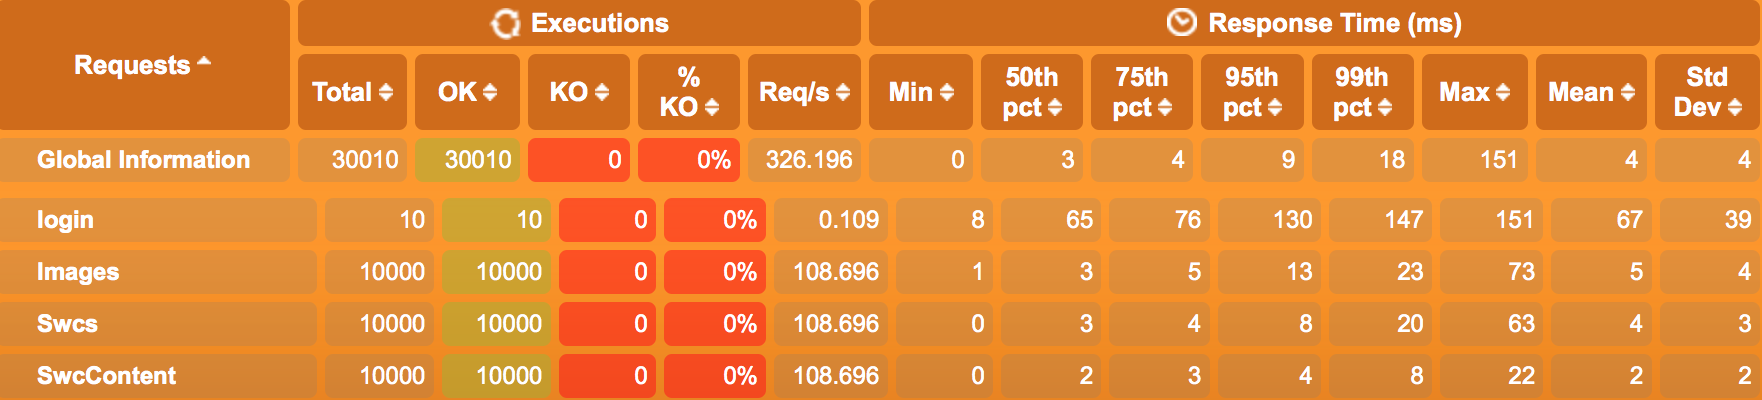
\includegraphics[width=108mm]{images/response}
\caption{请求响应时间,图中 Login 代表用户登录的请求,Images 代表获取用户原始图像列表相关 API 的响应时间,Swcs 代表用户对神经元结构进行操作的相关 API 的响应时间,SwcContent 代表用户获取结构脑胞体的响应时间。}
\label{response}
\end{figure}
